Ce chapitre détaille l'architecture technique du \textbf{Personal Behavior Anomaly Detection System (PBADS)} implémenté avec une architecture microservices.

\section{Vue d'ensemble du système}

PBADS suit une \textbf{architecture microservices} moderne avec 13 services distincts, permettant une séparation claire des responsabilités, une scalabilité élevée et une tolérance aux pannes. Cette architecture est organisée en quatre couches principales :

\begin{itemize}
    \item \textbf{Couche Frontend :} Service frontend (Thymeleaf) pour l'interface utilisateur
    \item \textbf{Couche API Gateway :} Point d'entrée unique pour toutes les requêtes client
    \item \textbf{Couche Infrastructure :} Services de support (Eureka, Config Server, Kafka, PostgreSQL, Redis, MLflow)
    \item \textbf{Couche Services Métier :} Services métier spécialisés (Auth, Data, Model, Inference, Alert, Monitoring, Recommendation)
\end{itemize}

\begin{figure}[H]
    \centering
    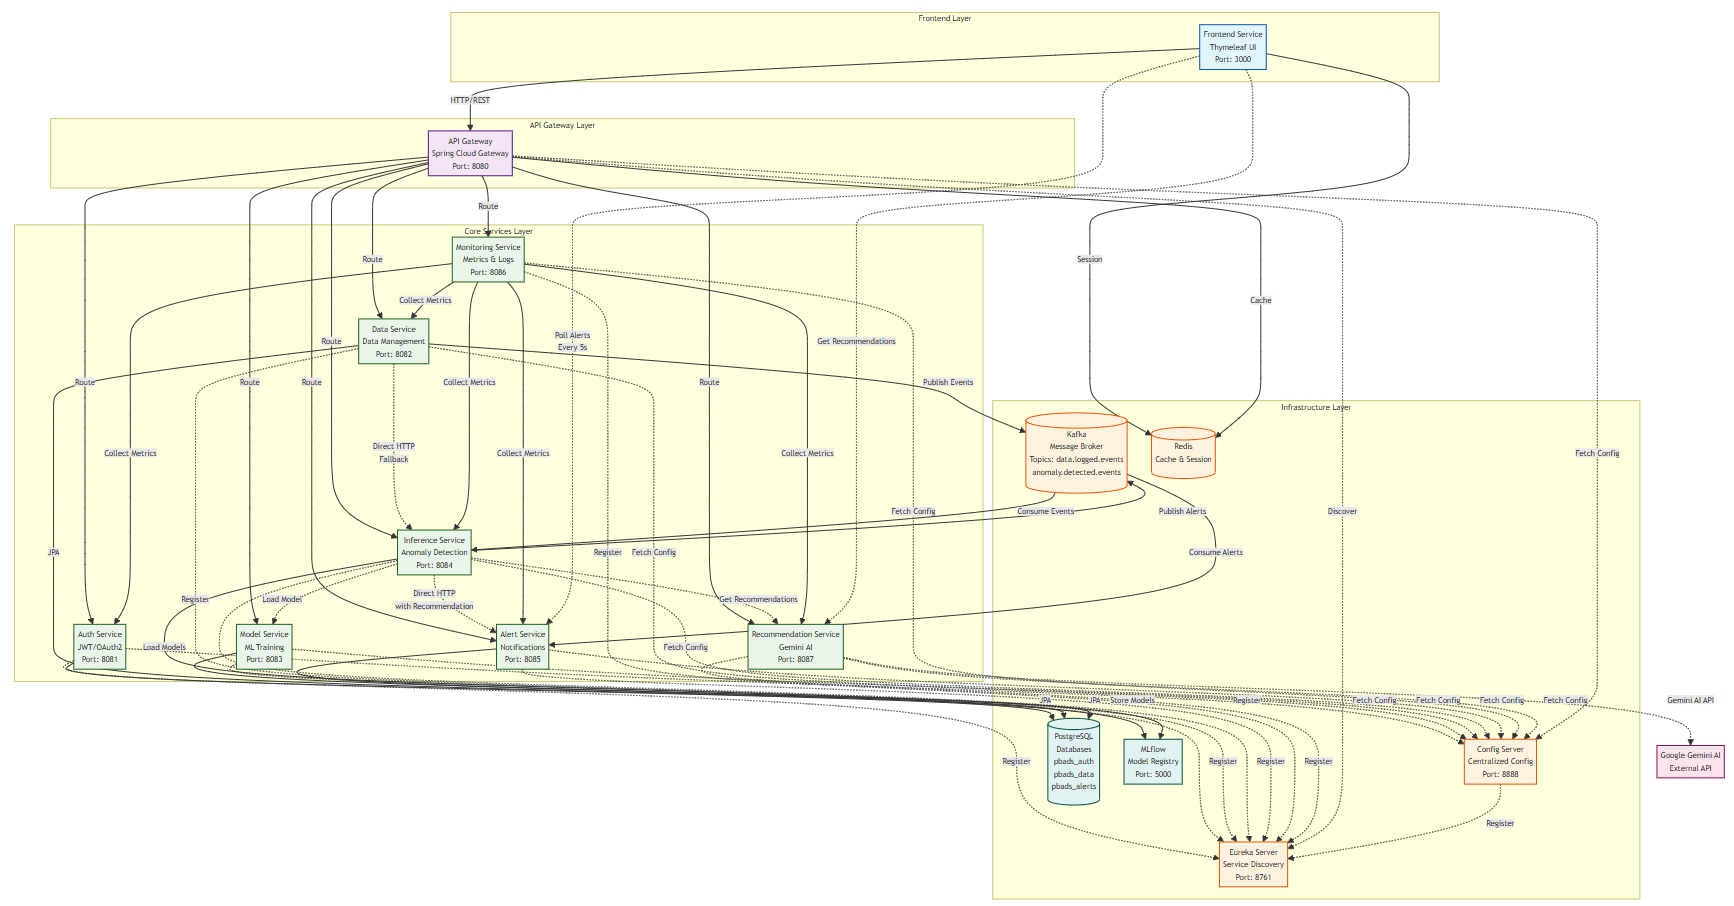
\includegraphics[width=\textwidth]{Figures/pbadsarchitecture/pbadsarchitecture.jpg}
    \caption{Architecture microservices du système PBADS}
    \label{fig:architecture_microservices}
\end{figure}

\textbf{Composants de l'architecture :}

\begin{itemize}
    \item \textbf{Frontend Service (Port 3000) :} Interface utilisateur développée avec Thymeleaf et Chart.js
    \item \textbf{API Gateway (Port 8080) :} Point d'entrée unique avec routage et authentification
    \item \textbf{Eureka Server (Port 8761) :} Service de découverte et registre des microservices
    \item \textbf{Config Server (Port 8888) :} Gestion centralisée de la configuration
    \item \textbf{Kafka :} Broker de messagerie pour la communication asynchrone entre services
    \item \textbf{PostgreSQL :} Bases de données relationnelles (une par service pour l'isolation des données)
    \item \textbf{Redis :} Cache et gestion de session
    \item \textbf{MLflow (Port 5000) :} Suivi des expériences ML et versioning des modèles
\end{itemize}

\section{Couche Services Métier}

\subsection{Auth Service (Port 8081)}

Le service d'authentification gère toutes les opérations d'authentification, d'autorisation et de gestion des utilisateurs.

\textbf{Fonctionnalités principales :}
\begin{itemize}
    \item Génération et validation de tokens JWT (HS512)
    \item Inscription et connexion des utilisateurs
    \item Chiffrement des mots de passe avec BCrypt
    \item Contrôle d'accès basé sur les rôles (ADMIN, USER)
    \item Opérations CRUD sur les utilisateurs (Admin uniquement)
    \item Activation/désactivation des comptes
\end{itemize}

\textbf{Base de données :} PostgreSQL (\texttt{pbads\_auth})

\textbf{Technologies :} Spring Security, JWT, BCrypt, Spring Data JPA

\subsection{Data Service (Port 8082)}

Le service de données gère toutes les opérations sur les données quotidiennes des utilisateurs.

\textbf{Fonctionnalités principales :}
\begin{itemize}
    \item Opérations CRUD sur les données quotidiennes
    \item Validation et persistance des données
    \item Publication d'événements Kafka (\texttt{data.logged.events})
    \item Appel HTTP direct vers Inference Service (mécanisme de fallback)
    \item Requêtes par utilisateur, date et plage de dates
\end{itemize}

\textbf{Modèle de données :}
\begin{itemize}
    \item User\_ID, Date, Wake\_Up\_Time
    \item Sleep\_Hours, Steps, Calories\_Burned
    \item Water\_Intake\_ml, Study\_Hours, Mood\_Score
\end{itemize}

\textbf{Base de données :} PostgreSQL (\texttt{pbads\_data})

\textbf{Technologies :} Spring Data JPA, Kafka Producer, Spring Cloud OpenFeign

\subsection{Model Service (Port 8083)}

Le service de modèles gère l'entraînement et la gestion des modèles d'apprentissage automatique.

\textbf{Fonctionnalités principales :}
\begin{itemize}
    \item Orchestration de l'entraînement des modèles (hybride Java/Python)
    \item Exécution de scripts Python pour l'entraînement
    \item Versioning et stockage des modèles
    \item Intégration MLflow pour le suivi des expériences
    \item Gestion des métadonnées des modèles
\end{itemize}

\textbf{Processus d'entraînement :}
\begin{enumerate}
    \item Chargement des données CSV depuis le chemin configuré
    \item Preprocessing des features (scaling, normalisation)
    \item Entraînement du modèle avec l'algorithme sélectionné
    \item Évaluation des performances du modèle
    \item Sauvegarde du modèle et des métadonnées sur disque
\end{enumerate}

\textbf{Technologies :} Python (scikit-learn), Java ProcessBuilder, MLflow

\subsection{Inference Service (Port 8084)}

Le service d'inférence effectue la détection d'anomalies en temps réel sur les données entrantes.

\textbf{Fonctionnalités principales :}
\begin{itemize}
    \item Consommateur Kafka pour \texttt{data.logged.events}
    \item Endpoint HTTP pour le traitement direct des données
    \item Chargement et inférence des modèles ML
    \item Détection basée sur des règles (fallback)
    \item Calcul du score d'anomalie (0-1)
    \item Détermination du niveau d'anomalie (NORMAL/LOW/MEDIUM/HIGH)
    \item Intégration avec Recommendation Service pour les recommandations IA
    \item Construction de résumés de données pour les prompts Gemini AI
    \item Producteur Kafka pour \texttt{anomaly.detected.events}
    \item Création d'alertes HTTP directes avec recommandations (fallback)
\end{itemize}

\textbf{Logique de détection :}
\begin{itemize}
    \item Tentative d'abord avec le modèle ML
    \item Fallback vers la détection basée sur des règles si le modèle est indisponible
    \item Seuils de règles : Sommeil (6-10h), Steps (≥5000), Eau (≥1500ml), Humeur (≥3/10), Étude (≤12h)
\end{itemize}

\textbf{Technologies :} Kafka Consumer/Producer, scikit-learn (via pont Java), Spring Cloud OpenFeign, RestTemplate

\subsection{Alert Service (Port 8085)}

Le service d'alertes gère les alertes générées à partir de la détection d'anomalies.

\textbf{Fonctionnalités principales :}
\begin{itemize}
    \item Création et persistance des alertes
    \item Consommateur Kafka pour \texttt{anomaly.detected.events}
    \item Endpoint HTTP pour la création directe d'alertes
    \item Gestion du statut des alertes (ACTIVE/ACKNOWLEDGED/RESOLVED)
    \item Requêtes d'alertes par utilisateur, statut, plage de dates
    \item Stockage des facteurs contributifs (JSON)
    \item Stockage des recommandations IA (champ TEXT pour les recommandations générées par Gemini)
\end{itemize}

\textbf{Modèle d'alerte :}
\begin{itemize}
    \item User ID, Date, Anomaly Score, Anomaly Level
    \item Message, Contributing Factors (JSON)
    \item \textbf{Recommendation} - Suggestions générées par l'IA Gemini
    \item Status, Created At timestamp
\end{itemize}

\textbf{Base de données :} PostgreSQL (\texttt{pbads\_alerts})

\textbf{Technologies :} Kafka Consumer, Spring Data JPA, Jackson JSON

\subsection{Recommendation Service (Port 8087)}

Le service de recommandations génère des recommandations personnalisées alimentées par l'IA en utilisant Google Gemini.

\textbf{Fonctionnalités principales :}
\begin{itemize}
    \item Intégration avec l'API Google Gemini AI
    \item Génération de recommandations personnalisées basées sur les données d'anomalie
    \item Réception de résumés de données avec détails d'anomalie et habitudes utilisateur
    \item Construction de prompts pour Gemini AI avec contexte
    \item Retour de recommandations actionnables pour améliorer les habitudes utilisateur
    \item Configuration via variables d'environnement (fichier .env)
    \item Gestion des erreurs pour la limitation de débit de l'API
\end{itemize}

\textbf{Endpoints :}
\begin{itemize}
    \item \texttt{POST /api/recommendations/generate} - Générer une recommandation avec corps de requête complet
    \item \texttt{GET /api/recommendations/user/\{userId\}?dataSummary=...} - Obtenir une recommandation pour un utilisateur
\end{itemize}

\textbf{Configuration :} Utilise \texttt{GEMINI\_API\_KEY} depuis les variables d'environnement ou le fichier .env

\textbf{Technologies :} Spring Boot Web, Spring WebFlux, Google Gemini API, dotenv-java, Eureka Client

\section{Communication entre services}

\subsection{Communication synchrone (HTTP/REST)}

La communication synchrone est utilisée pour les opérations nécessitant des réponses immédiates, telles que l'authentification utilisateur, la récupération de données et les appels directs entre services.

\textbf{Protocole :} HTTP/REST
\textbf{Client :} Spring Cloud OpenFeign
\textbf{Gateway :} Spring Cloud Gateway (Port 8080)
\textbf{Découverte de services :} Eureka Server

\textbf{Patterns de communication :}
\begin{itemize}
    \item \textbf{Frontend → Gateway → Auth Service :} Connexion, inscription, gestion des utilisateurs
    \item \textbf{Frontend → Gateway → Data Service :} Saisie de données, récupération de données
    \item \textbf{Frontend → Gateway → Alert Service :} Récupération d'alertes (polling toutes les 5 secondes)
    \item \textbf{Frontend → Gateway → Recommendation Service :} Recommandations du tableau de bord
    \item \textbf{Data Service → Inference Service :} Appel HTTP direct (fallback lorsque Kafka est indisponible)
    \item \textbf{Inference Service → Recommendation Service :} Génération de recommandations IA
    \item \textbf{Inference Service → Alert Service :} Création d'alertes HTTP directes avec recommandations
    \item \textbf{Inference Service → Model Service :} Chargement de modèles
\end{itemize}

\subsection{Communication asynchrone (Kafka)}

Kafka est utilisé pour la communication orientée événements, permettant le découplage et la scalabilité. Les services publient des événements sans attendre les consommateurs, permettant une meilleure tolérance aux pannes.

\textbf{Topics Kafka :}

\begin{table}[H]
\centering
\small
\renewcommand{\arraystretch}{1.4}
\begin{tabular}{|p{4cm}|p{3cm}|p{3cm}|p{5cm}|}
\hline
\textbf{Nom du Topic} & \textbf{Éditeur} & \textbf{Consommateur} & \textbf{Description} \\
\hline
\texttt{data.logged.events} & Data Service & Inference Service & Publié lorsque l'utilisateur soumet des données quotidiennes. Contient : userId, date, sleepHours, steps, caloriesBurned, waterIntakeMl, studyHours, moodScore, wakeUpTime \\
\hline
\texttt{anomaly.detected.events} & Inference Service & Alert Service & Publié lorsqu'une anomalie est détectée. Contient : userId, date, anomalyScore, anomalyLevel, message, contributingFactors, recommendation (générée par l'IA) \\
\hline
\end{tabular}
\caption{Topics Kafka du système PBADS}
\label{tab:kafka_topics}
\end{table}

\subsection{Mécanisme de fallback}

Le système implémente une \textbf{stratégie de communication en mode dual} pour la fiabilité :
\begin{itemize}
    \item \textbf{Primaire :} Kafka pour le traitement asynchrone des événements
    \item \textbf{Fallback :} Appels HTTP directs lorsque Kafka est indisponible
\end{itemize}

Cette approche garantit que le système continue de fonctionner même si Kafka est en panne, bien qu'avec un découplage réduit. Le Data Service et l'Inference Service tentent tous deux de publier sur Kafka mais effectuent également des appels HTTP directs comme mécanisme de sécurité.

\section{Sécurité et Authentification}

\subsection{JWT (JSON Web Tokens)}

L'authentification basée sur JWT permet une gestion sécurisée et stateless des sessions utilisateur. Les tokens sont signés avec l'algorithme HS512 et contiennent les informations de rôle de l'utilisateur.

\subsection{Contrôle d'accès basé sur les rôles}

Le système utilise un contrôle d'accès basé sur les rôles avec deux niveaux principaux :
\begin{itemize}
    \item \textbf{ADMIN :} Accès complet à toutes les fonctionnalités, y compris la gestion des utilisateurs
    \item \textbf{USER :} Accès aux fonctionnalités standard (tableau de bord, saisie de données, alertes, recommandations)
\end{itemize}

\section{Intégration Machine Learning}

\subsection{Algorithmes utilisés}

Le système utilise deux algorithmes principaux pour la détection d'anomalies :

\begin{itemize}
    \item \textbf{Isolation Forest :} Algorithme principal, excellent pour les données de grande dimension, rapide en entraînement et inférence
    \item \textbf{One-Class SVM :} Algorithme alternatif, efficace pour la détection d'anomalies non linéaires avec noyau RBF
\end{itemize}

\subsection{Processus d'inférence}

Lors de l'inférence, le modèle entraîné reçoit un vecteur de features représentant les habitudes d'une journée. Le modèle produit un score d'anomalie (0-1), qui est ensuite interprété comme :
\begin{itemize}
    \item \textbf{0.0 - 0.3 :} NORMAL - Comportement dans la plage normale
    \item \textbf{0.3 - 0.6 :} LOW - Déviation mineure de la normale
    \item \textbf{0.6 - 0.8 :} MEDIUM - Anomalie modérée détectée
    \item \textbf{0.8 - 1.0 :} HIGH - Anomalie significative nécessitant une attention
\end{itemize}

\section{Intégration Google Gemini AI}

Le système intègre Google Gemini AI pour générer des recommandations personnalisées. Lorsqu'une anomalie est détectée, l'Inference Service construit un résumé des données incluant les détails de l'anomalie et les habitudes de l'utilisateur, puis appelle le Recommendation Service. Ce service envoie un prompt contextuel à l'API Gemini, qui génère des recommandations personnalisées pour améliorer les habitudes de l'utilisateur.

\section{Conclusion}

L'architecture microservices mise en place pour PBADS offre une séparation claire des préoccupations entre les différents services, garantissant une maintenabilité optimale et une évolutivité adaptée aux besoins croissants du système. La sécurité multicouche, intégrant JWT et contrôle d'accès basé sur les rôles, assure une authentification robuste et un contrôle d'accès granulaire.

L'intégration Kafka pour la communication asynchrone et le mécanisme de fallback HTTP garantissent la résilience du système. L'intégration Google Gemini AI et les notifications en temps réel enrichissent l'expérience utilisateur tout en fournissant les outils nécessaires pour améliorer les habitudes de vie. Cette architecture constitue ainsi une base solide pour une solution de détection d'anomalies comportementales moderne et performante.
